% Created 2014-05-16 Fri 15:35
\documentclass[article]{jss}
\usepackage{amsmath,amsfonts}
\usepackage{float}
\usepackage{listings}\lstset{
keywordstyle=\color{blue},
commentstyle=\color{red},stringstyle=\color[rgb]{0,.5,0},
basicstyle=\ttfamily\small,
columns=fullflexible,
breaklines=true,
breakatwhitespace=false,
numbers=left,
numberstyle=\ttfamily\tiny\color{gray},
stepnumber=1,
numbersep=10pt,
backgroundcolor=\color{white},
tabsize=4,
showspaces=false,
showstringspaces=false,
xleftmargin=.23in,
frame=single,
basewidth={0.5em,0.4em},
literate={<-}{{\,$\leftarrow$\,}}1 {~}{{\,$\sim$\,}}1}
\usepackage{array}
\usepackage{dsfont}
\usepackage{tikz}
\usepackage{hyperref}
\usepackage{amsmath}
\usepackage{amssymb}
\usepackage{attrib}
\Plainauthor{C\'elia Touraine, Thomas A. Gerds, Pierre Joly}
\author{C\'elia Touraine\\University of Bordeaux \And Thomas A. Gerds\\University of Copenhagen \And Pierre Joly\\University of Bordeaux}
\title{Illness-Death Model for Interval-Censored Data: The \pkg{SmoothHazard} Package for \proglang{R}}
\Shorttitle{Illness-Death Model for Interval-Censored Data: The \pkg{SmoothHazard} Package for \proglang{R}}
\Keywords{illness-death model, interval-censored data, left-truncated data, survival model, proportional regression models, smooth transition intensities, Weibull, penalized likelihood, M-splines}
\Address{C\'elia Touraine\\Univ. Bordeaux\\ISPED\\Centre INSERM U-897-Epidemiologie-Biostatistique\\Bordeaux F-33000\\France\\E-mail: celia.touraine@isped.u-bordeaux2.fr\\URL: http://www.isped.u-bordeaux2.fr/}
\Abstract{The irreversible illness-death model describes the pathway from an
initial state to a absorbing state either directly or through an
intermediate state. This model is frequently used in medical
applications where the intermediate state represents illness and the
absorbing state represents death. In many studies, disease onset times
are not known exactly. This happens for example if the disease status
of a patient can only be assessed at regular visits. In this situation
the disease onset times are interval-censored. This article presents
the \pkg{SmoothHazard} package for \proglang{R}. It implements
algorithms for simultaneously fitting regression models to the three
transition intensities of an illness-death model where the transition
times to the intermediate state may be interval-censored and the all
event times can be right censored. The program parses the data
structure to find the corresponding contribution to the likelihood.
The three baseline hazard functions are modelled by Weibull
distributions, or by M-splines. For a given set of covariates, the
estimated transition intensities can be combined into predictions of
cumulative event probabilities and life expectancies.
}
\lstset{
keywordstyle=\color{blue},
commentstyle=\color{red},
stringstyle=\color[rgb]{0,.5,0},
basicstyle=\ttfamily\small,
columns=fullflexible,
breaklines=true,        % sets automatic line breaking
breakatwhitespace=false,    % sets if automatic breaks should only happen at whitespace
numbers=left,
numberstyle=\ttfamily\tiny\color{gray},
stepnumber=1,
numbersep=10pt,
backgroundcolor=\color{white},
tabsize=4,
showspaces=false,
showstringspaces=false,
xleftmargin=.23in,
frame=single,
basewidth={0.5em,0.4em}
}
\usepackage{graphicx}
\usepackage{array}
\date{\today}
\title{The SmoothHazard package for R: Fitting regression models to interval-censored observations of illness-death models}
\hypersetup{
 pdfkeywords={},
  pdfsubject={},
  pdfcreator={}}
\begin{document}

\maketitle
\section{Introduction}
\label{sec-1}

The irreversible illness-death model is a multi-state model which has
many applications in various areas of research, for example in the
medical field. The model describes the transitions from an initial
state (e.g., alive and disease-free) to an absorbing state (e.g.,
death) either directly or via an intermediate state (e.g., disease)
(Figure \ref{fig:1}). The transition intensities \(\alpha_{01}\),
\(\alpha_{02}\), and \(\alpha_{02}\) are positive functions of time which
can also depend on covariates.

\begin{figure}[htb]
\centering
\includegraphics[width=0.4\textwidth]{fig1.pdf}
\caption{\label{fig:1}The irreversible illness-death model}
\end{figure}

In some applications it happens for some or all subjects that the
transition times from the initial state to the intermediate state are
interval censored. This occurs for example when the status of the
intermediate state can only be determined at a sequence of visit
times. In this case, if a subject is diagnosed as diseased at one of
the visit times, say \(R\), then it is only known that the subject was
last seen disease-free at the previous visit time, say \(L\), and hence
the time of the onset of the disease is interval censored between \(L\)
and \(R\) for this subject. Furthermore, both the process of visit times
and the observation of the time of the transition into the absorbing
state are usually right censored, i.e., limited to the individual
follow-up period of the subjects. This yields a rather complex general
observational pattern, because for a subject who died without being
diagnosed as diseased at earlier visit times, it may or it may not be
possible to determine retrospectively if and when the subject became
diseased between the last visit time and the time of death.

The \pkg{SmoothHazard} package provides estimates of the baseline transition
intensities and of covariate effects when the data fall into one of
the 6 cases that are displayed in Figure \ref{fig:0}.
\begin{figure}[htb]
\centering
\includegraphics[width=0.5\textwidth]{obs-patterns.png}
\caption{\label{fig:0}Observational patterns that are recognized by \pkg{SmoothHazard}. The letters I and T denote the transition times into the intermediate and absorbing state, respectively. The letters E and C denote the start and end of follow-up, respectively, and the letters L and R the visit times between which the transition into the intermediate happened.}
\end{figure}
Thus, the case of left-truncated event times
(delayed entry) is covered, as well as the case where for some
subjects the transition time into the intermediate state is observed
exactly and for others it is interval censored.  Finally, the special
case is covered where for some or all subjects no intermediate
information is available about the disease status such that it is only
known whether or not the subjects became diseased between the start
and the end of follow-up. The latter occurs in Figure \ref{fig:0} when
\(E=L\) and \(R=\min(T,C)\) in cases 2. or 4.

To estimate covariate effects on the three transition intensities,
implemented are regression models which assume proportional transition
intensities and a non-homogeneous Markov process. The user chooses
between a fully parametric model where each of the baseline
intensities is described by the parameters of a Weibull distribution
and a semi-parametric model where the baseline intensities are left
unspecified and approximated by M-splines. For the parametric model,
the regression coefficients and Weibull parameters are estimated by
maximising the likelihood, for the semi-parametric model, the
coefficients of the M-splines and the regression coefficients are
estimated by maximising a penalized likelihood.

The package \pkg{SmoothHazard} then allows to do predictions of
transition probabilities, cumulative probabilities of event and 
life expectancies for a given set of covariates, 
based on estimated baseline transition intensities and on estimated 
covariates effects. 

If the exact transition times are observed, standard procedures like
those implemented, e.g. in the packages \pkg{survival}, \pkg{rms},
\pkg{etm}, \pkg{mstate} can be used to estimate transition
intensities, regression coefficients and functionals thereof
\citep[see][]{deWreede_Fiocco_Putter_2010, beyersmann2011competing}.
In particular, the regression coefficients can be estimated using Cox
partial likelihood \citep{coxpartial} without the need to model the
baseline intensities. However, when transition times to the
intermediate event are interval censored, it is generally not possible
to arrive at consistent estimates with the software provided by the
packages listed above. 
Indeed, the approach to handle subjects who died with unknown disease 
status, consists in artificially ending their follow-up 
at the last time they were seen without disease and subsequently 
treat them as right censored. 
However, this approach can lead to a systematic bias in the
estimates of transition intensities and of regression coefficients
\citep{Joly_Commenges_Helmer_Letenneur_2002, Leffondre_2013}. The bias
will be especially pronounced if the risk of death is higher for
diseased subjects than the risk of death for disease-free subjects.

The \pkg{msm} package \citep{Jackson_2010} allows to fit Markov
multi-state models to panel data where the status of the subjects is
known at a finite series of inspection times. As a special case the
setting includes the illness-death model and it can be used with
interval-censored disease times and exact death times. However, in
this package the likelihood is calculated using the Kolmogorov
differential equations that relate the transition probabilities and
the transition intensities and to make this work a time-homogeneity
assumption is made where all transition intensities are constant or
piecewise-constant between two successive observation times.

\subsubsection{Outline}
\label{sec-1-0-1}

The main functions of \pkg{SmoothHazard} are
\begin{itemize}
\item \code{idm} : for fitting illness-death regression models based on possibly interval-censored disease times and right censored times.
\end{itemize}
 A fitted illness-death model as produced
by \code{idm} can be used in the following functions to calculate predictions: 
\begin{itemize}
\item \code{predict.idm} : for estimating transition probabilities and cumulative probabilities of event for a given set of covariates;
\item \code{lifexpect} : for estimating life expectancies for a given set of covariates.
\end{itemize}

The \code{R} function \code{idm} is essentially an interface between 
the user
and \proglang{FORTRAN} programs which constitute the heart of the
package \pkg{SmoothHazard}.

Section 2 presents the model and the likelihood.
Section 3 presents the estimation methods.
Section 4 briefly presents predictions that can be made in an illness-death model. 
Section 5 provides some examples illustrating \pkg{SmoothHazard}.
\section{Model and likelihood}
\label{sec-2}

We consider an illness-death process \(X=(X(t),t \geq 0)\) which takes
values in \(\{0,1,2\}\) (Figure \ref{fig:1}). Subjects are initially
disease-free (\(X(0)=0\)) and may become diseased (transition \(0
\rightarrow 1\)) and die (transition \(1 \rightarrow 2\)), or die
directly without disease (transition \(0 \rightarrow 2\).)  \(X\) is
assumed to be a non-homogeneous Markov process which means that the
future evolution of the process \(\{X(t),t>s\}\) depends on the current
time \(s\) and only on the current state \(X(s)\). Thus, the distribution
of X is fully characterized by the set of transition probabilities:

\begin{equation*}
p_{hl}(s,t)=\mathbb{P}(X(t)=l|X(s)=h)\qquad hl \in \{01,02,12\}.
\end{equation*}

The transition probabilities are related to the instantaneous
transition intensities \(\alpha_{hl}\) shown in Figure \ref{fig:1} by
the relation: 
\begin{equation*}
\alpha_{hl}(t)=\lim_{\Delta t \to
0}\frac{p_{hl}(t,t+\Delta t)}{\Delta t}.
\end{equation*}


We introduce covariate effects separately for each transition through
proportional transition intensities regression models which are a
natural extension of the Cox proportional hazard model:
\begin{equation}
\alpha_{hl}(t|Z_{hli})=\alpha_{0,hl}(t)\exp\{\beta_{hl}^T Z_{hli}\};\qquad hl \in \{01,02,12\}.
\end{equation}
Here \(\alpha_{0,hl}\) are baseline transition intensities, \(Z_{hli}\)
are covariate vectors for subject \(i\) and \(\beta_{hl}\) are vectors of
regression parameters for transition \(h \rightarrow l\).

In the situation where the time to disease and the time to death are
not interval censored but either observed exactly or right censored,
the regression coefficients could be estimated by the partial likelihood
method without the need to specify and estimate the baseline hazard
functions \(\alpha_{0,hl}(t)\). For interval-censored transition times
to the intermediate state, the situation is more complex. It turns out
that we have to estimate all parameters simultaneously and that we
need a model for the baseline transition intensity functions. This can
be seen by inspecting the likelihood function.

For subject \(i\), denote the conditional disease-free survival function
by 
\begin{equation*}
S(t|Z_{01i},Z_{02i})=e^{- A_{01}(t|Z_{01i}) -A_{02}(t|Z_{02i})}
\end{equation*}
where \({A}_{hl}(.|Z_{hli})\) is the conditional cumulative intensity
function of transition \(h \rightarrow l\):
\begin{equation*}
{A}_{hl}(t|Z_{hli})=\int_0^t {\alpha}_{hl}(u|Z_{hli})du.
\end{equation*}
Note that
the conditional probability of surviving time \(t\) given a transition
into the intermediate state at time \(s\) is given by
$\exp\{-{A}_{12}(t|Z_{12i})+{A}_{12}(s|Z_{12i})\}.$

We allow that the event times are left truncated, i.e., that subjects
enter the study at the delayed entry time \(E>0\). The left truncation
condition \(X(E_{i})=0\) implies that subject \(i\) has survived in state
0 until time \(E_{i}\).

In addition to the covariate vectors \(Z_{01i},Z_{02i},Z_{12i}\) we
observe the vector \((E_i,L_i,R_i,\delta_{1i},\tilde T_i,\delta_{2i})\)
where \(\tilde T_i=\min(T_i,C_i)\) is the minimum between the transition
time into the absorbing state \(T_i\) and the right censoring time \(C_i\)
and \(\delta_{2i}=\mathds{1}\{T_i\le C_i\}\). Also, \(\delta_{1i}=1\) if we know
for sure that subject \(i\) was diseased between \(E_i\) and \(\tilde T_i\)
and \(\delta_{1i}=0\) otherwise. The visit times \(L_i\) and \(R_i\) are
defined by \(E_i\le L_i\le R_i\le \tilde T_i\) if \(\delta_{1i}=1\) and by
\(E_i\le L_i \le \tilde T_i, R_i=\infty\) if \(\delta_{1i}=0\). When the
transition time into the intermediate state is observed exactly, we
have \(\delta_{1i}=1\) and \(L_i=R_i\). In the latter case we also denote
\(I_i\) for the transition time into the intermediate state.

We now detail the likelihood contributions according to the different
observational patterns shown in Figure \ref{fig:0} in the special
case where there is no left truncation i.e. \(E_i=0\).
Left-truncated event times are taken into account by simply dividing 
the above
likelihood contributions by the term \({S(E_{i}|Z_{01i},Z_{02i})}\).
\begin{equation}\label{eq:1}
 \begin{split}
 %
 \text{case 1:}\quad {\cal L}_i & = S(C_i|Z_{01i},Z_{02i}) + \int_{L_i}^{C_i} S(u|Z_{01i},Z_{02i}) \alpha_{01}(u|Z_{01i}) \frac{e^{-{A}_{12}(C_i|Z_{12i})}}{e^{-{A}_{12}(u|Z_{12i})}}du \\
 %
 \text{case 2:}\quad {\cal L}_i & = \int_{L_i} ^{R_i} S(u|Z_{01i},Z_{02i}) \alpha_{01}(u|Z_{01i}) \frac{e^{-{A}_{12}(C_i|Z_{12i})}}{e^{-{A}_{12}(u|Z_{12i})}}du\\
 % 
 \text{case 3:}\quad {\cal L}_i & =  S(I_i|Z_{01i},Z_{02i}) \alpha_{01}(I_i|Z_{01i}) \frac{e^{-{A}_{12}(C_i|Z_{12i})}}{e^{-{A}_{12}(I_i|Z_{12i})}}\\
 %
 \text{case 4:}\quad {\cal L}_i & = \int_{L_i} ^{R_i} S(u|Z_{01i},Z_{02i}) \alpha_{01}(u|Z_{01i}) \frac{e^{-{A}_{12}(T_i|Z_{12i})}}{e^{-{A}_{12}(u|Z_{12i})}} \alpha_{12}(T_i|Z_{12i})du\\
 %
 \text{case 5:}\quad  {\cal L}_i & =  S(I_i|Z_{01i},Z_{02i}) \alpha_{01}(I_i|Z_{01i}) \frac{e^{-{A}_{12}(T_i|Z_{12i})}}{e^{-{A}_{12}(I_i|Z_{12i})}} \alpha_{12}(T_i|Z_{12i})\\ 
 %
 \text{case 6:}\quad {\cal L}_i & = S(T_i|Z_{01i},Z_{02i})\alpha_{02}(T_i|Z_{02i}) \\
  \qquad & + \int_{L_i}^{T_i} S(u|Z_{01i},Z_{02i}) \alpha_{01}(u|Z_{01i}) \frac{e^{-{A}_{12}(T_i|Z_{12i})}}{e^{-{A}_{12}(u|Z_{12i})}} \alpha_{12}(T_i|Z_{12i}) du \\
 %
 \end{split}
 \end{equation}
\section{Estimation}
\label{sec-3}

The \code{idm} function computes estimates for the three baseline
transition intensities and for the regression parameters using the
Levenberg-Marquardt's algorithm \citep{Levenberg_1944,Marquardt_1963}
to maximize the (penalized) likelihood.  The algorithm is a
combination of a Newton-Raphson algorithm and a gradient descent
algorithm (also known as the steepest descent algorithm). It has the
avantage of being more robust than the Newton-Raphson algorithm while
preserving its fast convergence property.

\subsection{Parametric estimation}
\label{sec-3-1}

In the default estimation method of function \code{idm}, a Weibull
parametrization for the baseline transition intensities is assumed: 
\begin{equation*}
\alpha_{0,hl}(t)= a_{hl} ~ b_{hl}^{a_{hl}} ~ t^{a_{hl}-1}; ~~~ hl \in
\{01,02,12\}.
\end{equation*}

where \(a_{hl}\) and \(\frac{1}{b_{hl}}\) are shape and scale
parameters.  The Weibull parameters estimates \(\hat{a}_{hl}\) and \(\hat{b}_{hl}\) and the
vectors of regression parameters estimates \(\hat \beta_{hl}\) are obtained
simultaneously by maximizing the likelihood which is the product over the
subjects' contributions according to equation \ref{eq:1}:


\begin{equation*}
{\cal{L}}(\beta_{01},\beta_{02},\beta_{12},a_{01},a_{02},a_{12},b_{01},b_{02},b_{12})
= \prod_{i=1}^n{\cal{L}}_i(\beta_{01},\beta_{02},\beta_{12},a_{01},a_{02},a_{12},b_{01},b_{02},b_{12}).
\end{equation*}


Confidence intervals for the regression parameters are obtained using
standard errors estimated by inverting the Hessian matrix of the
log-likelihood, that is the matrix of the second partial derivatives
of \(\log{\cal L}\) given in the previous display. Pointwise confidence intervals for
the baseline transition intensities are obtained using a
simulation-based approach explained below (section \ref{sec:CI}).
\subsection{Semi-parametric estimation}
\label{sec-3-2}
\label{sec:semi-para}

In situations where it is suspected that the Weibull distribution does
not fit the data very well one can think of extending the model and to
leave the baseline intensity functions completely unspecified, as in
the Cox regression model. Unfortunately, in interval-censored data
there is no direct analogue to the partial likelihood and the Breslow
estimator of the Cox model in right-censored data. 
The function \code{idm} implements a
semi-parametric model where the three baseline transition intensities
are approximated by linear combinations of M-splines. In this section
we explain the basic steps of the approach.

\subsubsection{The penalized likelihood}
\label{sec-3-2-1}

To control the smoothness of the estimated intensity functions, we
penalize the log-likelihood by a term which specificies the curvature
of the intensity functions. It is given by the square of the second
derivates. The penalized log-likelihood \((pl)\) is defined as:
\begin{equation}
\label{eq:77}
pl = l - \kappa_{01} \int {\alpha_{01} ^{''} }^2 (u|Z_{01}) du  - \kappa_{02} \int {\alpha_{02} ^{''} }^2 (u|Z_{02}) du
- \kappa_{12} \int {\alpha_{12} 
^{''} }^2 (u|Z_{12}) du
\end{equation}
where \(l\) is the log-likelihood and \(\kappa_{01}\), \(\kappa_{02}\) and
\(\kappa_{12}\) are three positive parameters which control the
trade-off between the data fit and the smoothness of the functions. It
is proposed that the penalization parameters are chosen by maximizing
a cross-validated likelihood score. Here, leave-one-out is appealing
as the result does not depend on the random seed as it would, e.g.,
for 10-fold cross-validation.  However, since leave-one-out requires
as many maximizations of the likelihood as there are subjects in the
data set, this can be computationally very expensive. To avoid
extremely long run times we have implemented the following algorithm:

Step 1. We ignore the covariates and use a grid search method to find
 the values for \((\kappa_{01}, \kappa_{02}, \kappa_{12})\) based on an
 approximiation of the leave-one-out log-likelihood score.  The
 approximation is equivalent to one step of the Newton-Raphson
 algorithm and reduces the number of calculations considerably. This
 approach was proposed by \citet{O'Sullivan_1988} for survival models
 and studied by \citet{Joly_Commenges_Helmer_Letenneur_2002} in an
 illness-death model
with interval censored data.

Step 2. We use the results of Step 1, i.e. the optimized value of
  \((\kappa_{01}, \kappa_{02}, \kappa_{12})\) to maximize the penalized
  likelihood \eqref{eq:77} with covariates. The parameters being
  maximized are the regression coefficients and the coefficients of
  the linear combinations of the M-splines defined below.
\subsubsection{M-splines}
\label{sec-3-2-2}

We use linear combinations of M-spline basis functions which are positive splines 
and variants of B-splines.
A family of M-spline functions of order \(k\), \(M_1,\ldots,M_n\) is
defined by a set of \(m\) knots where \(n=m+k-2\) \citep{Ramsay_1988}. We
consider only cubic M-splines of order \(k=4\). Denote by
\(t_{01}=(t_{01,1},\dots,t_{01,m_{01}})\) a sequence of \(m_{01}\) knots
used for 
approximating \(\alpha_{01}\) and by
\(t_{02}=(t_{02,1},\dots,t_{02,m_{02}})\) and
\(t_{12}=(t_{12,1},\dots,t_{12,m_{12}})\) similar sequences of knots for
approximating \(\alpha_{02}\) and \(\alpha_{12}\) respectively. We
denote by \(M_{hl}^T=M_{hl,1},\ldots,M_{hl,n_{hl}}\) the families of
\(n_{hl}\) cubic M-splines, with \(n_{hl}=m_{hl}+2\) and for \(hl \in
\{01,02,12\}\). 
 The baseline transition intensity \(\alpha_{0,hl}\) is approximated using
the following linear combination: 
\begin{equation*}
\tilde
\alpha_{0,hl}(t)=\sum_{i=1}^{n_{hl}} (a_{hl,i})^2 M_{hl,i}(t) 
\end{equation*}
where
\(a_{hl,i}\) are unkown parameters. The \(n_{hl}\) M-splines are integrated in order to
produce a family of monotone splines, these are called
I-splines. Thus, with each M-spline \(M_{hl,i}\) we associate an
I-spline \(I_{hl,i}\): 
\begin{equation*}
I_{hl,i}(t)=\int_{t_{hl,1}}^t M_{hl,i}(u) du.
\end{equation*}

For given values of the parameters \(a_{hl,i}\), we can approximate the
cumulative baseline transition intensities \(A_{hl}\) by a linear
combination of I-splines:

\begin{equation*}
\tilde A_{0,hl}(t)=\sum_{i=1}^{n_{hl}} (a_{hl,i})^2 I_{hl,i}(t).
\end{equation*}

Because M-splines are non-negative, the positivity constraint on
\((a_{hl,i})^2\) ensures that \(\tilde A_{0,hl}\) is monotone increasing.

\medskip

Confidence intervals of the regression parameters are obtained using
estimated standard errors which are obtained by inverting the Hessian
matrix of the penalized log-likelihood.

Confidence intervals for the transition intensities \(\alpha_{hl}(t)\)
are obtained using the Bayesian approach proposed in
\citet{O'Sullivan_1988} for survival analysis where the standard
errors are estimated by \(M_{hl}(t)^T H^{-1} M_{hl}(t)\) where \(H\)
denotes the Hessian matrix of the penalized log-likelihood.
\section{Predictions}
\label{sec-4}

Often in illness-death models the functions of interest are the
transition intensities.  However, other quantities (transition probabilities, cumulative probabilities and life
expectancies) which can be
expressed in terms of the transition intensities \citep{Touraine_2013}
may provide additional information and have a more natural
interpretation.

For example, given a set of covariates \(Z_{01,i},Z_{02,i},Z_{12,i}\)
for a subject \(i\) who is diseased at time \(s\), one could be interested
in probability to be still alive at some time \(t>s\), or in life
expectancy. Given a set of covariates \(Z_{01,j},Z_{02,j},Z_{12,j}\) for
a subject \(j\) who is diseased-free at time \(s\), one could be
interested in lifetime risk of disease or in healthy life expectancy
(expected remaining sojourn time in the healthy state). 
Since these quantities
can be written in terms of the transition intensities,
\pkg{SmoothHazard} provides estimates of them using estimates of the
transition intensities. Confidence intervals are
calculated using the simulation-based method immediately following.

\subsection{Confidence regions}
\label{sec-4-1}
\label{sec:CI}

A simulation based approach \citep{Mandel_2013} is used to calculate
confidence intervals for the transition intensities \(\alpha_{hl}(t)\)
in the parametric approach and for the other quantities of interest
in both parametric and semi-parametric approaches. 
To briefly outline how
it works, we generically denote by \(\theta\) the vector of all the
parameters that characterize the likelihood and by \(\hat\theta\) the
maximum (penalized) likelihood estimator.
\(\theta\) contains the Weibull parameters in the parametric model,
the spline parameters in the semi-parametric model
and the regression parameters in both models. 

We assume the asymptotic normality for the estimator \(\hat{\theta}\)
and denote by \(\hat{V}_{\hat{\theta}}\) the estimated covariance matrix
of \(\hat{\theta}\). We consider a multivariate normal distribution with
the parameters estimates as expectation and \(\hat{V}_{\hat{\theta}}\)
as covariance matrix. We generate \(n\) vectors (\(n=2000\) in practice)
from this distribution: \(\theta^{(1)},\ldots,\theta^{(n)}\).  Based on
them, we can calculate \(n\) values for the transition intensities:
\(\alpha_{hl}^{(1)}(t)\),\ldots,\(\alpha_{hl}^{(n)}(t)\), and therefore
\(n\) values for any quantity of interest written in terms of the
transition intensities.  The \(n\) values reflecting the sample
variation \citep{Aalen_Farewell_De_Angelis_Day_Gill_1997}, we order
them and the \(2.5^{\text{th}}\) and the \(97.5^{\text{th}}\) empirical
percentiles are then used as lower and upper confidence bounds for
95\% confidence intervals.  This procedure can be repeated for any
\(t\), so we can obtain pointwise confidence limits for
\({\alpha}_{hl}(.)\).
\section{Using SmoothHazard}
\label{sec-5}

\subsection{How to prepare the data}
\label{sec-5-1}
\begin{table}
\centering
\begin{tabular}{rm{18em}rrllll}
Case & Description & $\delta_1$ & $\delta_2$ & L & R & T & Remark\\
\hline
1 & No illness observed, right-censored death time & 0 & 0 & $L_i$ & $L_i$ & $C_i$ & $L_i\le C_i$\\
2 & Interval-censored ill time, right-censored death time & 1 & 0 & $L_i$ & $R_i$ & $C_i$ & $L_i<R_i\le C_i$\\
3 & Exact ill time, right-censored death time & 1 & 0 & $L_i$ & $L_i$ & $C_i$ & $L_i\le C_i$\\
4 & Interval-censored ill time, death time observed & 1 & 1 & $L_i$ & $R_i$ & $T_i$ & $L_i<R_i\le T_i$\\
5 & Exact ill time, death time observed & 1 & 1 & $L_i$ & $L_i$ & $T_i$ & $L_i\le T_i$\\
6 & No illness observed, death time observed & 0 & 1 & $L_i$ & $L_i$ & $T_i$ & $L_i\le T_i$\\
 &  &  &  &  &  &  & \\
\end{tabular}
\caption{Description of how the data set must be built to be understood by the \code{idm} function}
\label{tab:XX}
\end{table}

Table \ref{tab:XX} shows how the program interpretes the structure of the data
set. In all cases, \(L_i\) may be equal to the entry time. 
Some more details are necessary to distinguish the case where the
ill status is known at the last follow-up time for death from the case where
this is not possible. 

\begin{itemize}
\item In case 1, if \(L_i<C_i\) then it is assumed that the subject may
become ill between \(L_i\) and \(C_i\). If \(L_i=C_i\) it is assumed that
the subject is disease-free at time \(C_i\). In the latter case the
integral in the second term of the likelihood equals zero.
\item In case 6, if  \(L_i<T_i\) then it is assumed that the subject may
become ill between \(L_i\) and \(T_i\). If \(L_i=T_i\) it is assumed that
the subject is disease-free at time \(T_i\). In the latter case the
integral in the second term of the likelihood equals zero.
\end{itemize}
\subsection{Paquid study}
\label{sec-5-2}
In order to illustrate the functionality of the package we provide a
random subset containing data from 1000 subjects that were enrolled in
the Paquid study \citep{letenneur1999sex}, a large cohort study on
mental and physical aging.
\lstset{language=R,numbers=none}
\begin{lstlisting}
library(SmoothHazard)
data(Paq1000)
\end{lstlisting}
The population consists of subjects aged 65 years and older living in
Southwestern France. 
The event of interest is dementia and death without
dementia is a competing risk. Furthermore, the time to dementia onset
is interval censored between the diagnostic visit and the previous one 
and demented subjects are at risk of death.
Thus, subjects who died without being diagnosed as demented at their last visit 
may have become demented between last visit and death.

In this subset \texttt{186} subjects are diagnosed as demented
and \texttt{724} died from whom \texttt{597} without
being diagnosed as demented before. Because of interval censoring 
more than \texttt{186} should have been demented, more than
\texttt{127} should have been dead with dementia and
less than \texttt{597} should have been dead without dementia
(see Figure \ref{fig:2}).
\begin{center}
\begin{figure}
\centering
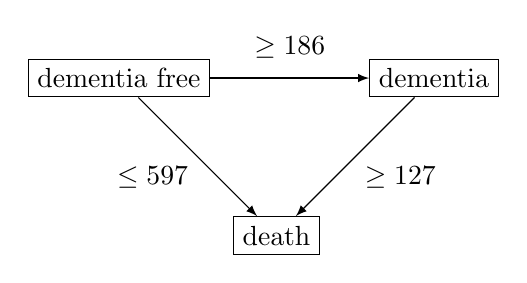
\begin{tikzpicture}[scale=1]
\node[draw] (nd) at (0,0) {dementia free};
\node[draw] (d) at (4,0) {dementia};
\node[draw] (dcd) at (2,-2) {death};
\draw[->,>=latex] (nd) -- (d)node[label=$\geq 186$,pos=0.5]{};
\draw[->,>=latex] (nd) -- (dcd) node[auto=right,pos=0.5]{$\leq 597$};
\draw[->,>=latex] (d) -- (dcd) node[auto=left,pos=0.5]{$\geq 127$};
\end{tikzpicture}
\caption{The exact number of transitions in the illness-death model with interval-censored time to disease is unknown: example of the \code{Paq1000} data set.}
\label{fig:2}
\end{figure}
\end{center}

Age is chosen as the basic time scale and subjects are dementia-free
(and alive) at entry into study.  Consequently, we need to deal with
left-truncated event times.

\lstset{language=R,numbers=none}
\begin{lstlisting}
head(round(Paq1000,1))
\end{lstlisting}

\begin{verbatim}
  dementia death    e    l    r    t certif gender
1        1     1 72.3 82.3 84.7 87.9      0      0
2        0     1 77.9 78.9 78.9 79.6      0      1
3        0     1 79.9 79.9 79.9 80.9      0      0
4        0     1 74.7 78.6 78.6 82.9      1      1
5        0     1 76.7 76.7 76.7 79.2      0      1
6        0     0 66.2 71.4 71.4 84.2      1      0
\end{verbatim}

Each row in the data corresponds to one subject.  The variables
\code{dementia} and \code{death} are  \(\delta_1\) and \(\delta_2\), 
the status variables for dementia and death.
The variable \code{e} contains ages of subjects at entry into
study. The variables \code{l} and \code{r} contain the left and right
endpoints of the censoring intervals.  For demented subjects, \code{r}
is the age at the diagnostic visit and \code{l} is the age at the
previous one.  For non demented subjects, \code{l} and \code{r} are
the age at the latest visit without dementia (\code{l}=\code{r}).  The
variable \code{t} is the age at death or at latest news on vital
status.  There are two binary covariates: \code{certif} for primary
school diploma (\texttt{762} with diploma and \texttt{238}
without diploma) and \code{gender} (\texttt{578} women and
\texttt{422} men).

The function \code{idm} computes estimates for the three transition
intensities \(\alpha_{01}(.)\), \(\alpha_{02}(.)\), \(\alpha_{12}(.)\) which
represents age-specific incidence rate of dementia, age-specific mortality
rate of dementia-free subjects and age-specific mortality rate of
demented subjects, respectively.  Proportional transition intensities
regression models allow for covariates on each transition.
Covariates are specified independently for the regression models of
the three transition intensities by the right hand side of the
respective formula \code{formula01}, \code{formula02} and
\code{formula12}.

Interval censoring and left truncation must be specified at the left
side of the formula arguments using the \code{Hist} function.  For
left-truncated data, the \code{entry} argument of \code{Hist} must
contain the vector of delayed entry times.  For interval-censored
data, the \code{time} argument of \code{Hist} must contain a list of
the left and right endpoints of the intervals.
The \code{data} argument contains the data frame in which to
interpret the variables of \code{formula01}, \code{formula02} and
\code{formula12}.
The left side of \code{formula12} argument does not need to be filled because all the data 
informations are already contained in \code{formula01} and \code{formula02}.
The left side of \code{formula12} argument is required only if we want the covariates 
impacting 
transition \(1 \rightarrow 2\) different from those impacting transition 
\(0 \rightarrow 2\).
\subsection{Fitting the illness-death model based on interval-censored data}
\label{sec-5-3}

The main function \code{idm} computes estimates for the three baseline
transition intensities and for the regression parameters of an
illness-death model.  The \code{intensities} argument by specifying
the form of the transition intensities allows to select either the
parametric or a semi-parametric estimation method :

\begin{itemize}
\item With the default value \code{"Weib"}, a Weibull distribution is
assumed for the baseline transition intensities and the parameters
are estimated by maximizing the log-likelihood;
\item With the \code{"Splines"} value, the baseline transition
intensities are approximated by linear combinations of
M-splines and the parameters are estimated by
maximizing the penalized log-likelihood.
\end{itemize}

We stop the iterations of the maximization algorithm when the differences 
between two consecutive
parameters values, log-likelihood values, and gradient values is small
enough.  The default convergence criteria are \(10^{-5}\), \(10^{-5}\) and
\(10^{-3}\) and can be changed by means of the \code{eps} argument.

We now illustrate how to fit the illness-death model to the 
\code{Paq1000} data set, based on 
interval-censored dementia times and exact death times.

\bigskip

In the following call, a Weibull parametrization is used for the three baseline 
transition intensities and we include two covariates on the transition to dementia,
one covariate on the transition from no dementia to death and no covariates 
on the transition from dementia to death. Note that in case of missing \code{formula12}
argument the covariates on the \(1 \rightarrow 2\) transition are the same as 
the ones specified in the  \code{formula02} argument.

\lstset{language=R,numbers=none}
\begin{lstlisting}
fit.weib <- idm(formula01=Hist(time=list(l,r),event=dementia,entry=e)~certif+gender,
		formula02=Hist(time=t,event=death,entry=e)~gender,
		formula12= ~ 1,
		data=Paq1000)
fit.weib
\end{lstlisting}

\begin{verbatim}
Call:
idm(formula01 = Hist(time = list(l, r), event = dementia, entry = e) ~ 
    certif + gender, formula02 = Hist(time = t, event = death, 
    entry = e) ~ gender, formula12 = ~1, data = Paq1000)

Illness-death model: Results of Weibull regression for the intensity functions.

number of subjects:  1000 
number of events '0 ->1':  186 
number of events '0 ->2' or '0 -> 1 -> 2':  724 

             coef SE.coef     HR          CI      Wald  p.value
certif_01 -0.4117  0.1827 0.6625 [0.46;0.95]  5.077537  0.02424
gender_01 -0.2621  0.1561 0.7694 [0.57;1.04]  2.818281  0.09320
gender_02  0.6712  0.1144 1.9565 [1.56;2.45] 34.449070 < 0.0001

               Without cov  With cov
Log likelihood   -3075.308 -3053.648

Parameters of the Weibull distribution: 'S(t) = exp(-(b*t)^a)'
          transition 0 -> 1 transition 0 -> 2 transition 1 -> 2
shape (a)       11.12344747        8.82268030        6.44006723
scale (b)        0.01102198        0.01074539        0.01381268

----
Model converged.
number of iterations:  7 
convergence criteria: parameters= 0.00000000011 
                    : likelihood= 0.0000000023 
                    : second derivatives= 0.0000000000008
\end{verbatim}


The hazard ratios HR (\(\mathrm{e}^{\text{coef}}\)) have the usual interpretation, 
as in a parametric Cox regression model.

The three baseline transition intensity functions can be displayed as
functions of time, functions of age in our illustrative example 
(Figure \ref{fig:alpha_weib}).
\lstset{language=R,numbers=none}
\begin{lstlisting}
par(mgp=c(4,1,0),mar=c(5,5,5,5))
plot(fit.weib,conf.int=TRUE,lwd=3,citype="shadow",xlim=c(65,100), axis2.las=2,axis1.at=seq(65,100,5),xlab="Age (years)")
\end{lstlisting}

\begin{figure}[htb]
\centering
\includegraphics[width=0.7\textwidth]{transition-intensities-paq-weib.pdf}
\caption{\label{fig:alpha_weib}Baseline transition intensities estimated using the Weibull parametrization of the parametric approach}
\end{figure}

\bigskip

The other estimation option in the function \code{idm} permits to
relax the strict parametric assumptions of the Weibull regression
models. With the option \code{intensities="Splines"}, 
linear combinations of M-splines are
used to approximate the three baseline transition
intensities. Although this option implies a considerable amount of
extra computations (see Section \ref{sec:semi-para}), the call and the printed output are
very similar to the Weibull model:

\lstset{language=R,numbers=none}
\begin{lstlisting}
fit.splines <- idm(formula01=Hist(time=list(l,r),event=dementia,entry=e)~certif+gender,
		   formula02=Hist(time=t,event=death,entry=e)~gender,
		   formula12= ~ 1,
		   intensities="Splines",data=Paq1000)
fit.splines
\end{lstlisting}

\begin{verbatim}
 Error: is.null(entry) || all(entry < L) is not TRUE
Error: object 'fit.splines' not found
\end{verbatim}

Again, the estimated baseline transition intensities can conveniently
be visualized in a joint graph (Figure \ref{fig:alpha_splines}).

\lstset{language=R,numbers=none}
\begin{lstlisting}
par(mgp=c(4,1,0),mar=c(5,5,5,5))
plot(fit.splines,conf.int=TRUE,lwd=3,citype="shadow",xlim=c(65,100), axis2.las=2,axis1.at=seq(65,100,5),xlab="Age (years)")
\end{lstlisting}

\begin{figure}[htb]
\centering
\includegraphics[width=0.7\textwidth]{transition-intensities-paq-splines.pdf}
\caption{\label{fig:alpha_splines}Baseline transition intensities estimated using the splines approximation of the semi-parametric approach}
\end{figure}


\subsubsection{Semi-parametric estimation method: choice of smoothing parameters}
\label{sec-5-3-1}

Some optional arguments are specific to the semi-parametric approach
(when using the option \code{intensities="Splines"}):

\begin{itemize}
\item \code{n.knots} contains a vector (by default \code{c(7,7,7)})
specifying the number of knots on the \(0 \rightarrow 1\), \(0
  \rightarrow 2\) and \(1 \rightarrow 2\) transitions, respectively;
\item \code{knots} contains the choice of the knots placement (equidistant
by default or quantile-based placement) or a list of sequences of
knots for transitions \(0 \rightarrow 1\), \(0 \rightarrow 2\) and \(1
  \rightarrow 2\) respectively, to be specified by the user;
\item \code{CV} (FALSE by default) is set to TRUE for using approximate
leave-one-out cross-validation score to choose the smoothing
parameters \(\kappa_{01}\), \(\kappa_{02}\), \(\kappa_{12}\);
\item \code{kappa} contains the smoothing parameters if \code{CV=FALSE}
(arbitrary choice of the smoothing parameters \(\kappa_{01}\),
\(\kappa_{02}\), \(\kappa_{12}\)); the initial smoothing parameters for
the grid search method which maximize the approximate leave-one-out
cross-validation score if \code{CV=TRUE}.
\end{itemize}

By default the function \code{idm} selects equidistant sequences of 7
knots between the minimal and maximal event times (\code{e}, \code{l}
and \code{r} for \code{Paq1000}). There must be a knot before or at
the first time from which there are subjects at risk and after or at
the last time of transition. The current implementation of our program
requires a minimum of 4 knots for each transition intensitiy.


Consequently, the semi-parametric approach
requires much more information than the parametric one to achieve
convergence. The number of parameters to be estimated is larger, and
enough observation times on each transition are required to fit the
splines.  In particular, in data sets where few \(1 \rightarrow 2\)
transitions times are observed, we does not recommended this approach.
Increasing the number of knots does not deteriorate the estimates of
the transition intensities: this is because the degree of smoothing in
the penalized likelihood method is tuned by the smoothing parameters
\(\kappa_{01}\), \(\kappa_{12}\) and \(\kappa_{02}\).  On the other hand,
once a sufficient number of knots is established, there is no
advantage in adding more.  Moreover, the more knots, the longer the
running time.  Some numerical problem can arise, particularly for a
large number of knots. 
So it is recommended to start with a small number of
knots (e.g. 5 or 7) and increase the number of knots until the graph
of the transition intensities function remains unchanged (from our own
experience rarely more than 12 knots).

The default values for the smoothing parameters \(\kappa_{01}\), \(\kappa_{02}\), 
\(\kappa_{01}\), are suitable for the
\code{Paq1000} data set. However, these values can be expected to be
very different depending on time scale, number of subjects and number of knots. 
The cross-validation option can be used to find appropriate smoothing parameters.
However, the running time with cross-validation is very long and an empirical
technique can be preferred. It consists in repeating the \code{idm} running
trying different smoothing parameters.  After each estimation, the
transition intensities are plotted. 
If the curves seem too smooth, it may be useful
to reduce the smoothing parameter. Similarly, if the curves
are too wiggly, the smoothing parameter may be increased.
\subsection{Making predictions}
\label{sec-5-4}
A object as returned by the \code{idm} function 
can be used as argument of the \code{predict} function in
order to obtain transition probabilities, cumulative probabilities of event and 
life expectancies with confidence intervals. 
For example, the following call give predictions regarding 
a 70 years-old male subject who have primary school diploma, 
over a 10 years horizon: 

\lstset{language=R,numbers=none}
\begin{lstlisting}
pred <- predict(fit.weib,s=70,t=80,Z01=c(1,1),Z02=1)
x<-round(do.call("rbind",pred),2)
colnames(x) <- c("Probability","Lower","Upper")
x
\end{lstlisting}

\begin{verbatim}
Error in predict(fit.weib, s = 70, t = 80, Z01 = c(1, 1), Z02 = 1) : 
  object 'fit.weib' not found
Error in do.call("rbind", pred) : object 'pred' not found
Error in colnames(x) <- c("Probability", "Lower", "Upper") : 
  object 'x' not found
Error: object 'x' not found
\end{verbatim}

The covariates values must be specified in the \code{Z01}, \code{Z02} and \code{Z12} 
arguments in the same order as they were entered in the preceding \code{idm} call.

The ouput attributes are:
\begin{itemize}
\item for a dementia-free 70 years-old subject: 
\begin{itemize}
\item the probability of being still alive and dementia-free 10 years later \(p_{00}(70,80)\),
\item the probability of being still alive but demented 10 years later \(p_{01}(70,80)\),
\item the probability of dying in the next 10 years \(p_{02}(70,80)\) having been demented before (\(p_{02}^1(70,80)\)) or not (\(p_{02}^0(70,80)\)),
\item the absolute risk of dementia in the 10 years (10 years later, the subject may be dead or not) \(F_{01}(s,t)\),
\item the absolute risk of exit from the no dementia state in the 10 years \(F_{0 \scriptscriptstyle{\bullet}}(s,t)\) (due to either dementia or death);
\end{itemize}
\item for a demented 70 years-old subject: the probability of dying in the next 10 years \(p_{12}(s,t)\) or not \(p_{11}(s,t)\).
\end{itemize}

The following calls give life expectancies regarding 
a 80 years-old female subject who have primary school diploma based on the 
transition intensities estimates from respectively the parametric approach 
and the semi-parametric approach:
\lstset{language=R,numbers=none}
\begin{lstlisting}
LE.weib <- lifexpect(fit.weib,s=80,Z01=c(1,0),Z02=0)
x<-round(do.call("rbind",LE.weib),2)
colnames(x) <- c("LE","Lower","Upper")
x
\end{lstlisting}

\begin{verbatim}
Error in lifexpect(fit.weib, s = 80, Z01 = c(1, 0), Z02 = 0) (from lifexpect.R#2) : 
  object 'fit.weib' not found
Error in do.call("rbind", LE.weib) : object 'LE.weib' not found
Error in colnames(x) <- c("LE", "Lower", "Upper") : object 'x' not found
Error: object 'x' not found
\end{verbatim}

\lstset{language=R,numbers=none}
\begin{lstlisting}
 LE.splines <- lifexpect(fit.splines,s=80,Z01=c(1,0),Z02=0,CI=FALSE)
x<-round(do.call("rbind",LE.splines),2)
colnames(x) <- c("LE")
x
\end{lstlisting}

\begin{verbatim}
Error in lifexpect(fit.splines, s = 80, Z01 = c(1, 0), Z02 = 0, CI = FALSE) (from lifexpect.R#2) : 
  object 'fit.splines' not found
Error in do.call("rbind", LE.splines) : object 'LE.splines' not found
Error in colnames(x) <- c("LE") : object 'x' not found
Error: object 'x' not found
\end{verbatim}

The confidence intervals calculation may take time, especially using the splines estimates of the transition intensities.
To suppress this calculation, the \code{CI} argument must be set to \code{FALSE} (see above).
To reduce the computation time of the confidence intervals, the number of simulations 
can also be modified using the \code{nsim} argument 
(by default 2000 for the \code{predict} function and 1000 for the \code{lifexpect} function).

The output attributes of  the \code{lifexpect} function are:
\begin{itemize}
\item for a dementia-free 80 years-old subject:
\begin{itemize}
\item the life expectancy in state 0 (healthy life expectancy),
\item the life expectancy;
\end{itemize}
\item for a demented 80 years-old subject: the life expectancy.
\end{itemize}

\subsubsection{Warnings regarding predictions}
\label{sec-5-4-1}
\label{sec:warnings}    
Predictions using the splines estimates of the transition intensities
are not possible if involving times prior to the first knot or times
beyond the last knot.  Moreover, the life expectancies are calculated
using integration until infinity using the Weibull estimates and until
the last knot using the splines estimates.  Consequently, to calculate
life expectancies using the splines estimates, we implicitly assume
that the last knot time is the maximal time of death.  The above life
expectancies calculating from the Weibull estimates or the splines
estimates of the transition intensities are very close because the
follow-up period of the \code{Paq1000} data set is long.  However, in
other data sets this assumption may not hold anymore.  
For data sets with short follow-up period, it is possible 
to calculate quantities involving any time, even infinity like 
life expectancies. However, beyond the follow-up time, they are not 
based anymore
on estimations of the transition itensity functions but rather on 
extrapolations on them. Consequently, we do not recommend to do 
predictions involving times beyond the follow-up period.
Finally, to
avoid numerical problem in the predictions calculations, the first and
last knots  for all transitions must be the same or very close.

\section*{Acknowledgments}
This work was supported by the grant 2010 PRSP 006 01 from the \textit{Agence Nationale de la Recherche} 
for the MOBIDYQ project and by the \textit{Région Aquitaine}.

\bibliography{smoothhazard}
\end{document}